\documentclass{standalone}
\usepackage{tikz}
\usepackage{ctex,siunitx}
\usepackage{tkz-euclide}
\usepackage{amsmath}
\usetikzlibrary{patterns, calc}
\usetikzlibrary {decorations.pathmorphing, decorations.pathreplacing, decorations.shapes,}
\begin{document}
\small
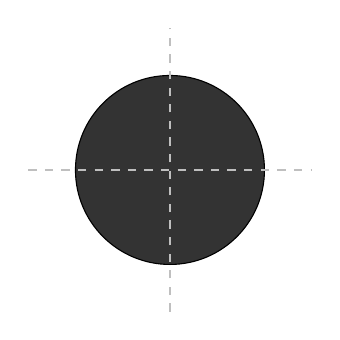
\begin{tikzpicture}[>=latex,scale=1.2]
  % \useasboundingbox(-1,1.2)rectangle(5,2.8);
  \draw[fill=black!80] (0,0) circle (1);
  \draw [dashed,lightgray](-1.5,0)--(1.5,0);         
  \draw [dashed,lightgray](0,-1.5)--(0,1.5); 
  \draw [ultra thick,green] plot[domain=-.7:.7, samples=100] function{-.5*sin(3.1416/0.7*x)};
  \end{tikzpicture}
\end{document}